\documentclass{tufte-handout}
\usepackage{pgfplots}
\usepackage[dvipsnames]{xcolor}
\usepackage{ulem}
\usepackage{subcaption}
\usepackage{amssymb, amsmath, pgfplots, tabularx, siunitx}
\usepackage{algorithm}
\usepackage{algorithmic}
\usepackage{makecell}
\usepackage{amsfonts}
\usepackage{thmtools}
\usepackage{enumitem}
\usepackage{adjustbox}
\usepackage{listings}
\usepackage{booktabs}
\pgfplotsset{compat = newest}

\usepackage{tikz}
\usetikzlibrary{shadings}
\usetikzlibrary{calc,arrows.meta}
\usetikzlibrary{shapes.misc}
\usetikzlibrary{shapes.geometric}
\usetikzlibrary{matrix}
\usetikzlibrary{positioning}
\usetikzlibrary{decorations.pathmorphing}
\usepackage[most]{tcolorbox}
\usepgfplotslibrary{colormaps,patchplots}

% Cores preservadas
\definecolor{wp-bg}{HTML}{FDF6EF}
\definecolor{wp-text}{HTML}{2D1B0E}
\definecolor{wp-primary}{HTML}{C24A3A}
\definecolor{wp-accent}{HTML}{D4952E}
\definecolor{wp-light}{HTML}{F0DECA}
\definecolor{wp-muted}{HTML}{C4A88A}
\definecolor{wp-dark}{HTML}{1A0F07}
\definecolor{wp-code}{HTML}{FDF2E4}

\pagecolor{wp-bg}
\color{wp-text}

\hypersetup{colorlinks=true,linkcolor=wp-primary,urlcolor=wp-accent}

\let\subsubsection\subsection

% Theorem environments
\declaretheorem[style=plain, name=Definition, numberwithin=section]{defn}
\declaretheorem[style=plain, name=Theorem, numberwithin=section]{thm}
\declaretheorem[style=plain, name=Lemma, numberwithin=section]{lem}
\declaretheorem[style=remark, name=Example, numberwithin=section]{exmp}
\declaretheorem[style=remark, name=Remark, numberwithin=section]{remark}

% Configuração do listings
\lstdefinestyle{pythonstyle}{
    language=Python,
    backgroundcolor=\color{wp-code},
    basicstyle=\ttfamily\small\color{wp-text},
    keywordstyle=\color{wp-primary}\bfseries,
    stringstyle=\color{wp-accent},
    commentstyle=\color{wp-muted}\itshape,
    numbers=left,
    numberstyle=\tiny\color{wp-muted},
    numbersep=8pt,
    breaklines=true,
    frame=single,
    rulecolor=\color{wp-muted!50},
    framerule=0.5pt,
    xleftmargin=15pt,
    showstringspaces=false
}
\lstset{style=pythonstyle}

\title{Machine Learning Notes \\ Chapter 3: Generalization and Regularization}
\author{Vitor N. Cabral de Oliveira\\ \href{mailto:vnco@cin.ufpe.br}{vnco@cin.ufpe.br}}
\date{\today}

\begin{document}
\maketitle
\begin{abstract}
    In Chapters 1 and 2, we built an engine capable of mapping inputs to outputs and optimizing its weights via gradient descent. However, a highly expressive model trained without constraints will simply memorize the training data, failing catastrophically on unseen examples. In this chapter, we address the core challenge of machine learning: \textit{Generalization}. We explore the bias-variance tradeoff, the modern phenomenon of double descent, and the mathematical foundations of regularization techniques like L2 Weight Decay, Dropout, and Batch Normalization.
\end{abstract}

\newpage
\hypersetup{linkcolor=wp-text}
\tableofcontents
\hypersetup{linkcolor=wp-primary}
\newpage

\section{Optimization vs. Generalization}

In machine learning, there is a strict distinction between the training set and the test set. The model's ability to perform well on data it has never seen before is called \textbf{generalization}.

Recall our goal: we want to minimize the \textit{expected risk} (the true error over all possible data drawn from the distribution). Since we don't have access to the true distribution, we minimize the \textit{empirical risk} (the error over our training dataset $\mathcal{D}$). 

If our model has millions of parameters, it can drive the training loss to zero by memorizing the exact input-output pairs. But memorization is not learning. When presented with a new input, a memorizing model has no underlying understanding of the data's structure and will output garbage.

\begin{marginfigure}[-2.0cm]
\centering
\begin{tcolorbox}[colback=wp-light, colframe=wp-accent, title=\textbf{Intuition: The Cramming Student}]
Imagine a student preparing for a math exam by memorizing the answer key of a single practice sheet. They score perfectly on that sheet but fail the actual exam, which contains unseen problems. A model that memorizes the training set is this student: perfect on the data it saw, useless on new data. \textit{Generalization} is the ability to solve problems the student has never seen.
\end{tcolorbox}
\end{marginfigure}

\subsection{The Bias-Variance Decomposition}

To understand generalization mathematically, we look at the expected generalization error of a model for a target $y$ and prediction $\hat{y}$. For squared error loss, the expected error can be decomposed into three parts:

\[
\mathbb{E}[(y - \hat{y})^2] = \underbrace{(\mathbb{E}[\hat{y}] - y)^2}_{\text{Bias}^2} + \underbrace{\mathbb{E}[(\hat{y} - \mathbb{E}[\hat{y}])^2]}_{\text{Variance}} + \underbrace{\sigma^2}_{\text{Irreducible Error}}
\]

\begin{marginfigure}[-4.0cm]
\centering
\resizebox{0.97\marginparwidth}{!}{%
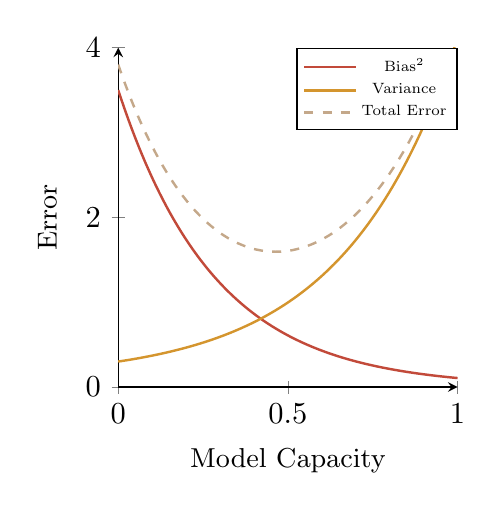
\begin{tikzpicture}[scale=1.1]
    \begin{axis}[
        width=5.5cm, height=5.5cm, 
        xlabel={Model Capacity}, 
        ylabel={Error}, 
        domain=0:1, 
        samples=100,
        xmin=0, xmax=1,
        ymin=0, ymax=4,
        xtick={0, 0.5, 1},
        ytick={0, 2, 4},
        axis x line=bottom, 
        axis y line=left, 
        enlargelimits=false,
        xlabel style={at={(axis description cs:0.5,-0.15)}, anchor=north, font=\small},
        ylabel style={at={(axis description cs:-0.15,0.5)}, anchor=south, font=\small},
        legend style={
            font=\scriptsize, 
            nodes={scale=0.7, transform shape}, 
            inner sep=2pt, 
            at={(1,1)}, 
            anchor=north east
        }]
        % Bias^2: Decreases with capacity
        \addplot[wp-primary, thick] {3.5 * exp(-3.5*x)}; 
        
        % Variance: Increases with capacity
        \addplot[wp-accent, thick] {0.1 + 0.2 * exp(3*x)}; 
        
        % Total Error: U-shape
        \addplot[wp-muted, thick, dashed] {3.5 * exp(-3.5*x) + 0.1 + 0.2 * exp(3*x)}; 
        
        \legend{Bias$^2$, Variance, Total Error};
    \end{axis}
\end{tikzpicture}}
\caption{The classical Bias-Variance Tradeoff. Total error has a minimum at an optimal intermediate capacity.}
\label{fig:bias_variance_tradeoff}
\end{marginfigure}

\begin{itemize}[leftmargin=*, itemsep=2pt]
    \item \textbf{Bias:} The error from erroneous assumptions in the model. A low-capacity model (e.g., a linear model trying to fit a sinusoidal wave) has high bias. This is \textit{underfitting}.
    \item \textbf{Variance:} The error from sensitivity to small fluctuations in the training set. A high-capacity model (e.g., a deep neural network) can fit any noise in the data, meaning its predictions will vary wildly if trained on different subsets of data. This is \textit{overfitting}.
    \item \textbf{Irreducible Error:} The noise inherent to the data generation process. No model can reduce this.
\end{itemize}

The classical goal of machine learning was to find the "sweet spot" in Figure~\ref{fig:bias_variance_tradeoff}—the model capacity where the sum of bias and variance is minimized.

To see the tradeoff concretely, consider fitting polynomials to a handful of noisy points sampled from a smooth curve. The degree of the polynomial plays the role of model capacity.

\begin{figure}[htbp]
\centering
\resizebox{\textwidth}{!}{%
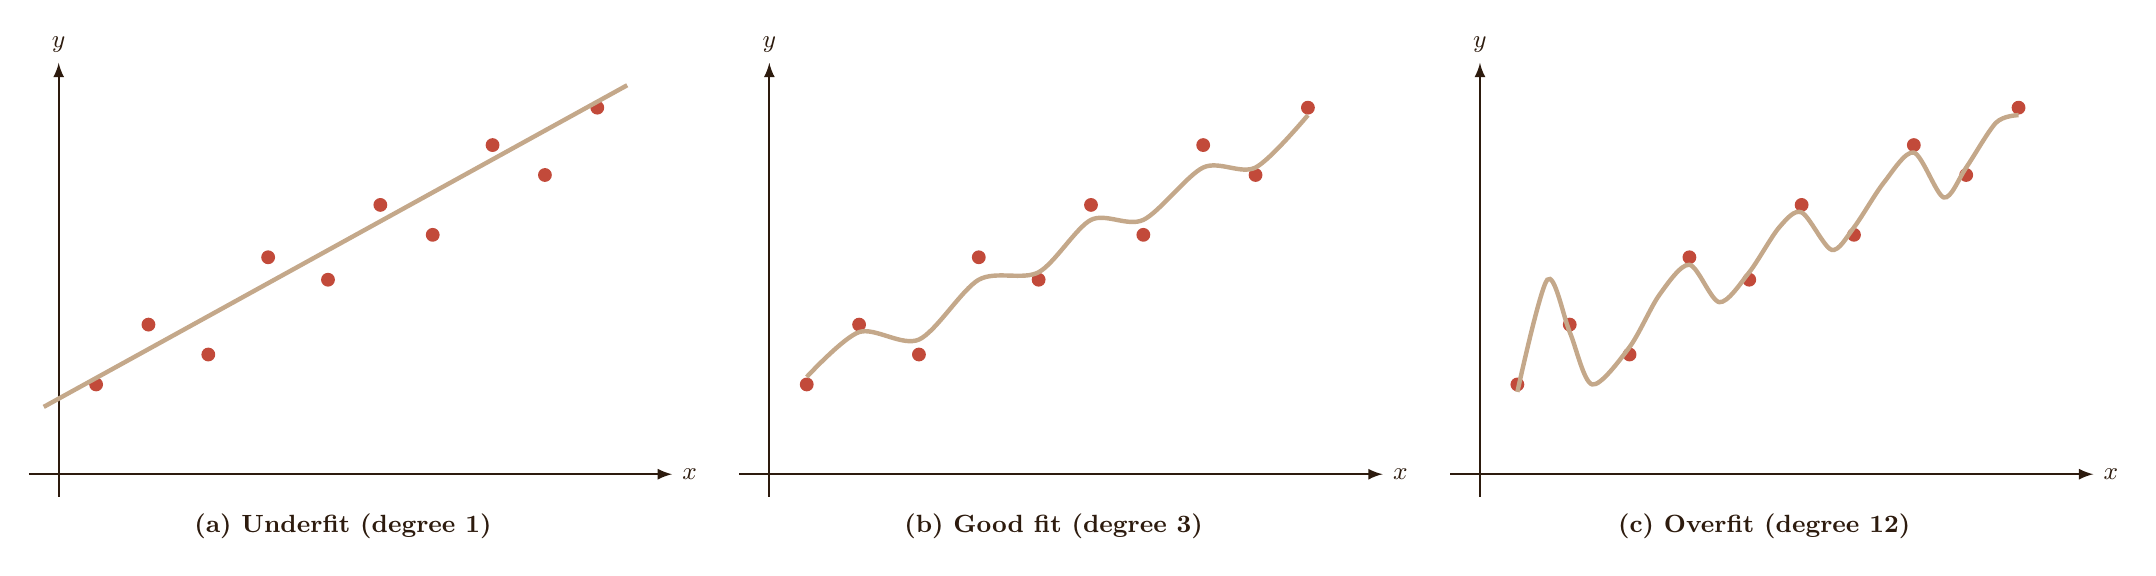
\begin{tikzpicture}[scale=0.95, >=latex, thick]
    % Data points (shared by all three panels)
    \def\datapoints{(0.5,1.2) (1.2,2.0) (2.0,1.6) (2.8,2.9) (3.6,2.6) (4.3,3.6) (5.0,3.2) (5.8,4.4) (6.5,4.0) (7.2,4.9)}
    
    % --- Panel (a): Underfit (degree 1) ---
    \begin{scope}[shift={(0, 0)}]
        \draw[->, wp-text] (-0.4, 0) -- (8.2, 0) node[right, font=\small] {$x$};
        \draw[->, wp-text] (0, -0.3) -- (0, 5.5) node[above, font=\small] {$y$};
        \draw[wp-primary] plot[only marks, mark=*, mark size=2.2pt] coordinates \datapoints;
        \draw[wp-muted, ultra thick] (-0.2,0.9) -- (7.6,5.2);
        \node[wp-text, font=\small\bfseries] at (3.8, -0.7) {(a) Underfit (degree 1)};
    \end{scope}
    
    % --- Panel (b): Good fit (degree 3) ---
    \begin{scope}[shift={(9.5, 0)}]
        \draw[->, wp-text] (-0.4, 0) -- (8.2, 0) node[right, font=\small] {$x$};
        \draw[->, wp-text] (0, -0.3) -- (0, 5.5) node[above, font=\small] {$y$};
        \draw[wp-primary] plot[only marks, mark=*, mark size=2.2pt] coordinates \datapoints;
        \draw[wp-muted, ultra thick, smooth] plot coordinates {
            (0.5,1.3) (1.2,1.9) (2.0,1.8) (2.8,2.6) (3.6,2.7) (4.3,3.4) (5.0,3.4) (5.8,4.1) (6.5,4.1) (7.2,4.8)
        };
        \node[wp-text, font=\small\bfseries] at (3.8, -0.7) {(b) Good fit (degree 3)};
    \end{scope}
    
    % --- Panel (c): Overfit (degree 12) ---
    \begin{scope}[shift={(19, 0)}]
        \draw[->, wp-text] (-0.4, 0) -- (8.2, 0) node[right, font=\small] {$x$};
        \draw[->, wp-text] (0, -0.3) -- (0, 5.5) node[above, font=\small] {$y$};
        \draw[wp-primary] plot[only marks, mark=*, mark size=2.2pt] coordinates \datapoints;
        \draw[wp-muted, ultra thick, smooth] plot coordinates {
            (0.5,1.1) (0.9,2.6) (1.2,1.9) (1.5,1.2) (2.0,1.7) (2.4,2.4) (2.8,2.8) (3.2,2.3)
            (3.6,2.7) (4.0,3.3) (4.3,3.5) (4.7,3.0) (5.0,3.3) (5.4,3.9) (5.8,4.3) (6.2,3.7)
            (6.5,4.1) (6.9,4.7) (7.2,4.8)
        };
        \node[wp-text, font=\small\bfseries] at (3.8, -0.7) {(c) Overfit (degree 12)};
    \end{scope}
\end{tikzpicture}}
\caption{Polynomial fits to the same noisy data. (a) A degree-1 line cannot capture the curvature---high bias, low variance. (b) A degree-3 polynomial tracks the underlying trend---low bias, moderate variance. (c) A degree-12 polynomial wiggles through \emph{every} point, fitting the noise itself---low bias but very high variance: it will perform poorly on new data.}
\label{fig:bias_variance_fits}
\end{figure}

\begin{exmp}[Bias, Variance, and Fit]
The three panels of Figure~\ref{fig:bias_variance_fits} tell a quantitative story. Suppose the true function is $y = x^{1.2} + \text{noise}$. Evaluated on the same ten points:
\begin{enumerate}[leftmargin=*, itemsep=2pt]
    \item \textbf{Underfit:} The straight line misses the curvature systematically. Averaged over many training sets, its predictions land near a \emph{consistently wrong} value---large Bias$^2$, small Variance.
    \item \textbf{Good fit:} The cubic follows the trend. Its average prediction is close to the truth (small Bias$^2$) and does not change much across training sets (moderate Variance).
    \item \textbf{Overfit:} The high-degree polynomial reproduces the training noise almost exactly. On a different training set, the wild wiggles would move dramatically---small Bias$^2$ but large Variance. The test error explodes even though the training error is $\approx 0$.
\end{enumerate}
\end{exmp}

\subsection{The Modern Reality: Double Descent}

Classical statistics suggests that as model capacity increases past the sweet spot, the test error will rise indefinitely (overfitting). However, modern Deep Learning defies this dogma. If we make the model \textit{massively} over-parameterized (far more parameters than data points), the test error drops again and often reaches its lowest point!

\begin{figure}[htbp]
\centering
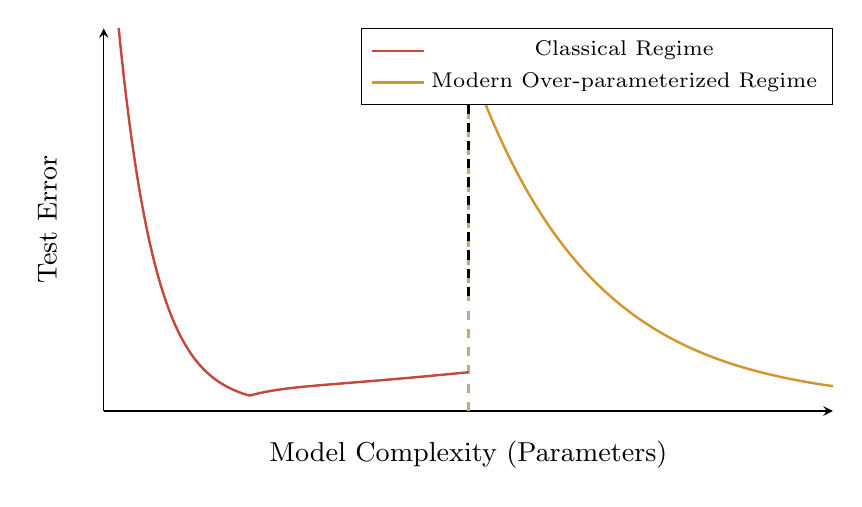
\begin{tikzpicture}[scale=1.1]
    \begin{axis}[
        width=10cm, height=6cm,
        xlabel={Model Complexity (Parameters)}, 
        ylabel={Test Error}, 
        domain=0:10, 
        samples=200,
        xmin=0, xmax=10,
        ymin=0, ymax=5,
        xtick=\empty,
        ytick=\empty,
        axis x line=bottom, 
        axis y line=left, 
        enlargelimits=false,
        xlabel style={at={(axis description cs:0.5,-0.05)}, anchor=north, font=\small},
        ylabel style={at={(axis description cs:-0.05,0.5)}, anchor=south, font=\small},
        legend style={font=\scriptsize, at={(1,1)}, anchor=north east}
    ]
        % Interpolation Threshold (where train error hits 0)
        \draw[wp-muted, dashed, thick] (axis cs:5, 0) -- (axis cs:5, 4.5);
        \node[wp-muted, font=\scriptsize\bfseries, align=center] at (axis cs:5, 4.8) {Interpolation\\Threshold};

        % Classical U-curve (up to threshold)
        \addplot[wp-primary, thick, domain=0:5] {0.2 + 3.5*abs(x-2)*exp(-1.5*x) + 0.1*abs(x-2)};
        
        % Modern descent (after threshold)
        \addplot[wp-accent, thick, domain=5:10] {4.5*exp(-0.6*(x-5)) + 0.1};
        
        % Smooth connection
        \addplot[black, thick, dashed] coordinates {(5,1.5) (5, 4.5)};
        
        \legend{Classical Regime, Modern Over-parameterized Regime};
    \end{axis}
\end{tikzpicture}
\caption{The Double Descent phenomenon. Past the interpolation threshold (where train error becomes zero), increasing model complexity actually decreases test error.}
\label{fig:double_descent}
\end{figure}

This phenomenon is known as \textbf{Double Descent} (Fig.~\ref{fig:double_descent}). Neural networks don't just memorize; they search for the \textit{simplest} function that interpolates the data. This modern finding explains why we can train LLMs with billions of parameters without catastrophic overfitting. However, explicit regularization is still required to stabilize training and guide the model toward these well-behaved solutions.

\section{Regularization Techniques}

\textbf{Regularization} encompasses any technique designed to reduce generalization error, often at the cost of increased training error. We constrain the hypothesis space.

\subsection{L2 Regularization (Weight Decay)}

The simplest form of regularization adds a penalty term to the loss function that discourages large weights. For a loss $\mathcal{L}_0$ and weight vector $\mathbf{w}$, the regularized loss is:

\[
\mathcal{L} = \mathcal{L}_0 + \frac{\lambda}{2} \|\mathbf{w}\|_2^2
\]

\begin{marginfigure}[-2.0cm]
\centering
\begin{tcolorbox}[colback=wp-light, colframe=wp-accent, title=\textbf{Bayesian View of L2}]
From a probabilistic perspective, L2 regularization is equivalent to Maximum A Posteriori (MAP) estimation assuming a Gaussian prior over the weights. We are telling the model: "Assume most weights should be close to zero unless the data strongly suggests otherwise."
\end{tcolorbox}
\end{marginfigure}

When we compute the gradient, the L2 term adds $\lambda \mathbf{w}$ to the update rule. This causes the weights to "decay" towards zero at every step:
\[
\mathbf{w} \leftarrow \mathbf{w} - \eta (\nabla \mathcal{L}_0 + \lambda \mathbf{w}) = \mathbf{w}(1 - \eta\lambda) - \eta \nabla \mathcal{L}_0
\]
Geometrically, L2 constraint creates a hypersphere in weight space. The optimizer is forced to find a solution that lies inside this hypersphere, preferring distributed, small weights over a few dominant ones.

\begin{exmp}[Weight Decay in Action]
Consider a single weight with $\eta = 0.1$, $\lambda = 0.5$, and suppose the data gradient is zero ($\nabla \mathcal{L}_0 = 0$)---the model has already fit the training set. The update rule becomes
\[
w \leftarrow w(1 - \eta\lambda) = w \times (1 - 0.05) = 0.95\,w.
\]
Starting from $w = 2.0$, the weight follows $2.0 \to 1.9 \to 1.805 \to 1.715 \to \dots$, shrinking by $5\%$ each step. Even without any data pressure, the weight inexorably decays toward zero. The decay rate is controlled entirely by the product $\eta\lambda$: the same update can be implemented by multiplying weights by $(1-\eta\lambda)$ after every step---which is why the technique is also called \emph{weight decay}. When the data gradient is nonzero, the decay and the data term compete, and the weight settles where the two balance.
\end{exmp}

\subsection{Dropout}

While L2 operates on the loss function, Dropout operates directly on the network architecture. During training, a random fraction $p$ of neurons in a layer is set to zero (dropped) during the forward pass. 

\begin{lstlisting}[caption={Dropout implementation in \texttt{mini\_nn/nn\_utils.py}.}]
import numpy as np

class Dropout:
    def __init__(self, p=0.5):
        self.p = p # Probability of dropping a neuron
        
    def __call__(self, x, training=True):
        if not training:
            return x # During inference, use all neurons
        
        # Generate binary mask. Neurons are kept with probability (1-p)
        mask = (np.random.rand(*x.shape) > self.p) / (1.0 - self.p)
        return x * mask
\end{lstlisting}

\begin{marginfigure}[-4.0cm]
\centering
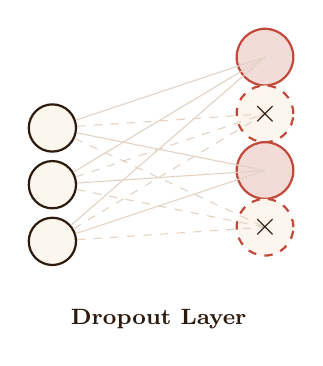
\begin{tikzpicture}[scale=0.9, >=latex]
    % Input Layer
    \foreach \i in {1,2,3} {
        \node[circle, draw=wp-text, thick, fill=wp-bg, minimum size=0.6cm] (i\i) at (0, 2-\i*0.8) {};
    }
    
    % Hidden Layer (With Dropout)
    \foreach \i in {1,...,4} {
        \pgfmathsetmacro{\fillval}{ifthenelse(\i==2 || \i==4, "wp-bg", "wp-primary!20")}
        \pgfmathsetmacro{\drawval}{ifthenelse(\i==2 || \i==4, "dashed", "solid")}
        
        \draw[draw=wp-primary, thick, fill=\fillval, \drawval] (3, 3-\i*0.8) circle (0.4cm);
        
        % Connections
        \foreach \j in {1,2,3} {
            \pgfmathsetmacro{\conval}{ifthenelse(\i==2 || \i==4, "dashed", "solid")}
            \draw[wp-muted!50, \conval] (i\j) -- (3, 3-\i*0.8);
        }
    }
    
    % X Marks for dropped
    \node[wp-text, font=\large\bfseries] at (3, 1.4) {$\times$};
    \node[wp-text, font=\large\bfseries] at (3, -0.2) {$\times$};
    
    \node[wp-text, font=\footnotesize\bfseries] at (1.5, -1.5) {Dropout Layer};
\end{tikzpicture}
\caption{Dropout during training. Active paths are solid; dropped paths are dashed.}
\label{fig:dropout}
\end{marginfigure}

Dropout prevents \textit{co-adaptation}. Without dropout, neurons might learn to rely heavily on the output of a specific upstream neuron. If that upstream neuron fails, the downstream neuron fails. By randomly dropping neurons, the network is forced to learn redundant representations—multiple paths must encode the same information.

During inference (testing), no neurons are dropped. However, because only $(1-p)$ neurons were active during training, we must scale the activations during inference by $(1-p)$ to maintain the expected output magnitude (or, as in the code above, scale by $1/(1-p)$ during training so inference needs no scaling).

\subsection{Batch Normalization (BN)}

Deep networks suffer from \textit{internal covariate shift}: as weights update, the distribution of inputs to deeper layers changes continuously, forcing those layers to constantly adapt. Batch Normalization stabilizes this by explicitly normalizing the inputs of each layer.

For a mini-batch $\mathcal{B} = \{x_1, \dots, x_m\}$, BN calculates the mean $\mu_{\mathcal{B}}$ and variance $\sigma_{\mathcal{B}}^2$:
\[
\mu_{\mathcal{B}} = \frac{1}{m}\sum_{i=1}^m x_i, \qquad \sigma_{\mathcal{B}}^2 = \frac{1}{m}\sum_{i=1}^m (x_i - \mu_{\mathcal{B}})^2
\]
It then normalizes the inputs:
\[
\hat{x}_i = \frac{x_i - \mu_{\mathcal{B}}}{\sqrt{\sigma_{\mathcal{B}}^2 + \epsilon}}
\]
Finally, it applies a learnable scale $\gamma$ and shift $\beta$:
\[
y_i = \gamma \hat{x}_i + \beta
\]

The transformation is easiest to visualize as a three-stage pipeline applied elementwise to every activation:

\begin{figure}[htbp]
\centering
\resizebox{\textwidth}{!}{%
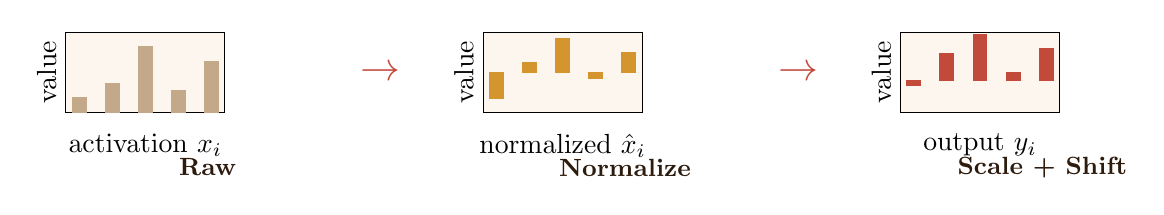
\begin{tikzpicture}[scale=1.0, >=latex]
    % Stage 1: Raw activations
    \begin{scope}[shift={(0, 0)}]
        \begin{axis}[
            width=3.6cm, height=2.6cm,
            ybar=0, bar width=5pt,
            ymin=0, ymax=1.1,
            xlabel={activation $x_i$}, ylabel={value},
            xtick=\empty, ytick=\empty,
            axis background/.style={fill=wp-bg},
            nodes near coords={}, 
        ]
            \addplot[fill=wp-muted, draw=wp-muted] coordinates {(0,0.2) (1,0.4) (2,0.9) (3,0.3) (4,0.7)};
        \end{axis}
        \node[wp-text, font=\small\bfseries] at (1.8, -0.7) {Raw};
    \end{scope}
    
    \node[wp-primary, font=\Large\bfseries] at (4.0, 0.5) {$\to$};
    
    % Stage 2: Normalized
    \begin{scope}[shift={(5.3, 0)}]
        \begin{axis}[
            width=3.6cm, height=2.6cm,
            ybar=0, bar width=5pt,
            ymin=-0.6, ymax=0.6,
            xlabel={normalized $\hat{x}_i$}, ylabel={value},
            xtick=\empty, ytick=\empty,
            axis background/.style={fill=wp-bg},
        ]
            \addplot[fill=wp-accent, draw=wp-accent] coordinates {(0,-0.4) (1,0.15) (2,0.5) (3,-0.1) (4,0.3)};
        \end{axis}
        \node[wp-text, font=\small\bfseries] at (1.8, -0.7) {Normalize};
    \end{scope}
    
    \node[wp-primary, font=\Large\bfseries] at (9.3, 0.5) {$\to$};
    
    % Stage 3: Scaled/shifted
    \begin{scope}[shift={(10.6, 0)}]
        \begin{axis}[
            width=3.6cm, height=2.6cm,
            ybar=0, bar width=5pt,
            ymin=-0.6, ymax=0.9,
            xlabel={output $y_i$}, ylabel={value},
            xtick=\empty, ytick=\empty,
            axis background/.style={fill=wp-bg},
        ]
            \addplot[fill=wp-primary, draw=wp-primary] coordinates {(0,-0.1) (1,0.5) (2,0.85) (3,0.15) (4,0.6)};
        \end{axis}
        \node[wp-text, font=\small\bfseries] at (1.8, -0.7) {Scale + Shift};
    \end{scope}
\end{tikzpicture}}
\caption{The BatchNorm pipeline: raw activations $\to$ zero-mean/unit-variance $\to$ learnable affine transform $\gamma \hat{x} + \beta$. The learnable parameters restore whatever mean and scale the layer needs, while the normalization itself keeps the distribution stable.}
\label{fig:bn_pipeline}
\end{figure}

The learnable $\gamma$ and $\beta$ are crucial: if the optimal behavior were to leave the activations untouched, BN can learn $\gamma = \sqrt{\sigma^2 + \epsilon}$ and $\beta = \mu$ to recover the identity, so the layer is never \emph{forced} to normalize away useful signal.

\begin{lstlisting}[caption={BatchNorm implementation in \texttt{mini\_nn/nn\_utils.py}.}]
import numpy as np

class BatchNorm:
    def __init__(self, dim, momentum=0.9, eps=1e-5):
        self.gamma = np.ones(dim)       # learnable scale
        self.beta = np.zeros(dim)       # learnable shift
        self.momentum = momentum
        self.eps = eps
        self.running_mean = np.zeros(dim)   # EMA, used at inference
        self.running_var = np.ones(dim)

    def __call__(self, x, training=True):
        if not training:
            # Inference: use the population statistics (EMA)
            x_hat = (x - self.running_mean) / np.sqrt(self.running_var + self.eps)
            return self.gamma * x_hat + self.beta

        # Training: use the current mini-batch statistics
        batch_mean = x.mean(axis=0)
        batch_var = x.var(axis=0)
        x_hat = (x - batch_mean) / np.sqrt(batch_var + self.eps)

        # Update the EMA of the population statistics
        self.running_mean = self.momentum * self.running_mean + (1 - self.momentum) * batch_mean
        self.running_var  = self.momentum * self.running_var  + (1 - self.momentum) * batch_var

        return self.gamma * x_hat + self.beta
\end{lstlisting}

\begin{remark}[Training vs. Inference in BN]
During training, BN uses the batch statistics. During inference (evaluation), we cannot rely on a single batch's statistics. Instead, PyTorch maintains an exponential moving average (EMA) of the mean and variance across all training batches, and uses these population estimates during testing. This is why calling \texttt{model.eval()} is critical in PyTorch.
\end{remark}

Beyond stabilizing training, BN acts as a mild regularizer. The noise injected by the batch statistics (since the mean/variance are slightly different for each mini-batch) slightly perturbs the network, similar to Dropout, improving generalization.

\subsection{Early Stopping}

The simplest, yet highly effective, form of regularization. We monitor the validation loss during training. As long as the validation loss decreases, training continues. Once the validation loss plateaus or starts to rise (indicating the model has begun to memorize noise), training is halted.

\begin{lstlisting}[caption={Pseudo-code for Early Stopping.}]
best_val_loss = float('inf')
patience = 5
epochs_no_improve = 0

for epoch in range(max_epochs):
    train_loss = train_one_epoch(model)
    val_loss = evaluate(model, val_data)
    
    if val_loss < best_val_loss:
        best_val_loss = val_loss
        save_model(model) # Save the best weights
        epochs_no_improve = 0
    else:
        epochs_no_improve += 1
        if epochs_no_improve >= patience:
            print("Early stopping triggered.")
            break
            
load_best_model(model)
\end{lstlisting}

Early stopping effectively limits the optimization algorithm's capacity to overfit. By stopping early, we constrain the trajectory of the optimizer in the weight space, landing in a wider, flatter minimum (which generalizes better) rather than a sharp, deep minimum (which overfits).

The behavior this exploits is visible in almost every training run: the training loss keeps decreasing monotonically, while the validation loss eventually turns around and climbs. Early stopping identifies that turning point.

\begin{figure}[htbp]
\centering
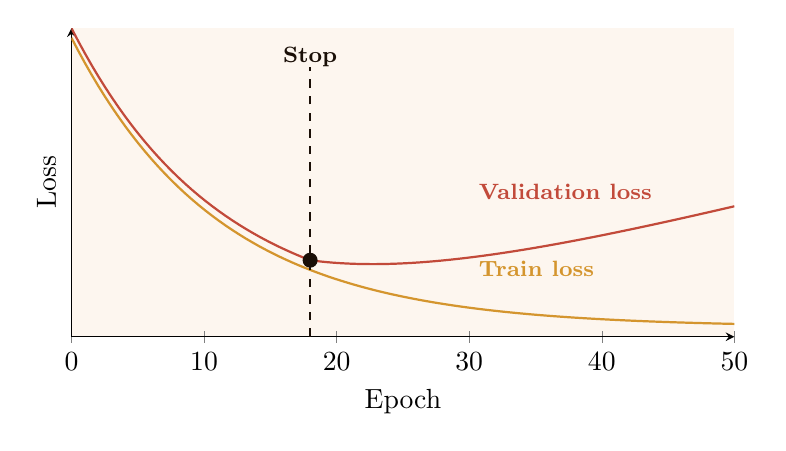
\begin{tikzpicture}[scale=1.0, >=latex]
    \begin{axis}[
        width=10cm, height=5.5cm,
        xlabel={Epoch},
        ylabel={Loss},
        domain=0:50,
        samples=100,
        xmin=0, xmax=50,
        ymin=0, ymax=1.6,
        xtick={0,10,20,30,40,50},
        ytick=\empty,
        axis x line=bottom,
        axis y line=left,
        enlargelimits=false,
        axis background/.style={fill=wp-bg}
    ]
        % Training loss (monotonically decreasing)
        \addplot[wp-accent, thick, domain=0:50] {1.5*exp(-0.09*x) + 0.05};
        % Validation loss (decreases then increases)
        \addplot[wp-primary, thick, domain=0:50] {1.5*exp(-0.09*x) + 0.1 + 0.35*max(0,(x-18))/20};
        % Stop marker
        \draw[wp-dark, dashed, thick] (axis cs:18, 0) -- (axis cs:18, 1.4);
        \filldraw[wp-dark] (axis cs:18, {1.5*exp(-0.09*18) + 0.1}) circle (2.5pt);
        \node[wp-dark, font=\footnotesize\bfseries, anchor=south] at (axis cs:18, 1.35) {Stop};
        \node[wp-accent, font=\footnotesize\bfseries, anchor=west] at (axis cs:30, 0.35) {Train loss};
        \node[wp-primary, font=\footnotesize\bfseries, anchor=west] at (axis cs:30, 0.75) {Validation loss};
    \end{axis}
\end{tikzpicture}
\caption{Training vs. validation loss. The training loss (gold) falls steadily, but the validation loss (terracotta) reaches a minimum around epoch 18 and then rises as the model starts to memorize noise. Early stopping halts training at that minimum, before overfitting begins.}
\label{fig:early_stopping}
\end{figure}

\subsubsection{A Summary of Regularization Techniques}

\begin{table}[htbp]
\centering
\small
\begin{tabularx}{\textwidth}{@{}>{\raggedright\arraybackslash}p{2.3cm}X X X@{}}
\toprule
\textbf{Technique} & \textbf{Mechanism} & \textbf{Training effect} & \textbf{Inference effect} \\
\midrule
\textbf{L2 / Weight Decay} & penalty $\frac{\lambda}{2}\|\mathbf{w}\|^2$ in the loss & weights shrink toward zero & unchanged \\
\textbf{Dropout} & random neurons zeroed per step & forces redundant representations & no drops; scaled activations \\
\textbf{BatchNorm} & normalize + scale/shift per batch & stable distributions; mild noise & uses population EMA \\
\textbf{Early Stopping} & halt when validation loss rises & shorter training, flatter minima & unchanged \\
\bottomrule
\end{tabularx}
\caption{Summary of the four regularization techniques covered in this chapter. They act on different components---the loss, the architecture, the activations, or the training schedule---but all serve the same goal: reduce generalization error.}
\label{tab:regularization_summary}
\end{table}

\subsubsection{Exercises}

\begin{enumerate}[leftmargin=*, itemsep=4pt]
    \item Using the decomposition $\mathbb{E}[(y-\hat{y})^2] = \text{Bias}^2 + \text{Variance} + \sigma^2$, explain in one sentence each why a low-capacity and a high-capacity model generalize poorly.
    \item A weight $w = 4.0$ is trained with weight decay $\lambda = 0.1$ and learning rate $\eta = 0.01$. If the data gradient is zero, write down the first three weight values.
    \item Dropout scales activations by $1/(1-p)$ during training. Why does this make inference (no scaling) consistent? What would happen to the output magnitude if the scaling were omitted?
    \item BatchNorm maintains an EMA of batch statistics. Why can't the final batch's statistics be used directly at inference time?
    \item In the double descent curve, what happens to the \emph{training} error after the interpolation threshold? Why does the \emph{test} error keep decreasing in that regime?
    \item Early stopping requires a separate validation set. How would you detect overfitting if you only had access to the training set? What is the risk of doing so?
    \item For each of the four regularization techniques, state which component of the learning process (loss, architecture, activations, or schedule) it modifies.
\end{enumerate}

\begin{remark}[The Transition to Architecture]
We now know how to build models (Chapter 1), how to train them (Chapter 2), and how to prevent them from memorizing (Chapter 3). However, applying a generic MLP to images results in an explosion of parameters and the loss of spatial structure. In Chapter 4, we will introduce \textit{Inductive Bias} through Convolutional Neural Networks (CNNs), tailoring our architectures to the structure of the data.
\end{remark}

\end{document}